
To conduct realistic coexistence experiments with real LTE-U traffic, 
we implemented LTE-U protocol stack 
using programmable software defined radio on two different platforms, 
i.e., Sora~\cite{sora}, operating at 5 GHz and bladeRF~\cite{bladeRF}, operating at 2.4 GHz. 
Our LTE-U implementation consists of a LTE transmitter, a Wi-Fi sniffer and a controller.
The architecture is depicted in Figure~\ref{fig:platform}.
The LTE transmitter PHY is implemented in Ziria~\cite{stewart2015ziria} according to Release 8 specification of LTE, and tested using commercial LTE dongles. 
Ziria is a customzied programming language designed
to make writing PHY layer code simpler.  
We have a customized translator that 
can translate Ziria code into C code.
The MAC layer of the LTE-U module is written in C. 


The Wi-Fi sniffer monitors Wi-Fi packets over the air and estimates Wi-Fi channel usage.
The Wi-Fi sniffer is implemented on 64bit Ubuntu 15.10
with Linux kernel version 4.2.0. 
It is written in C/C++ with 1500 lines of code. 
Base on Wi-Fi channel usage, the controller adjusts LTE-U on/off duty cycle. 
The LTE-U base station transmits LTE signals according to the on/off duty cycle. 
We illustrate the prototype with a picture in Figure~\ref{fig:testbed}.
The controller and LTE-U base station are connected by
Ethernet cable. 
The control message is transmitted over UDP socket. 
We have also released the entire source code as open source~\cite{OpenLTEU} to enable the wider community to further build on our initial study.



\begin{figure}[!htb]
 \centering
     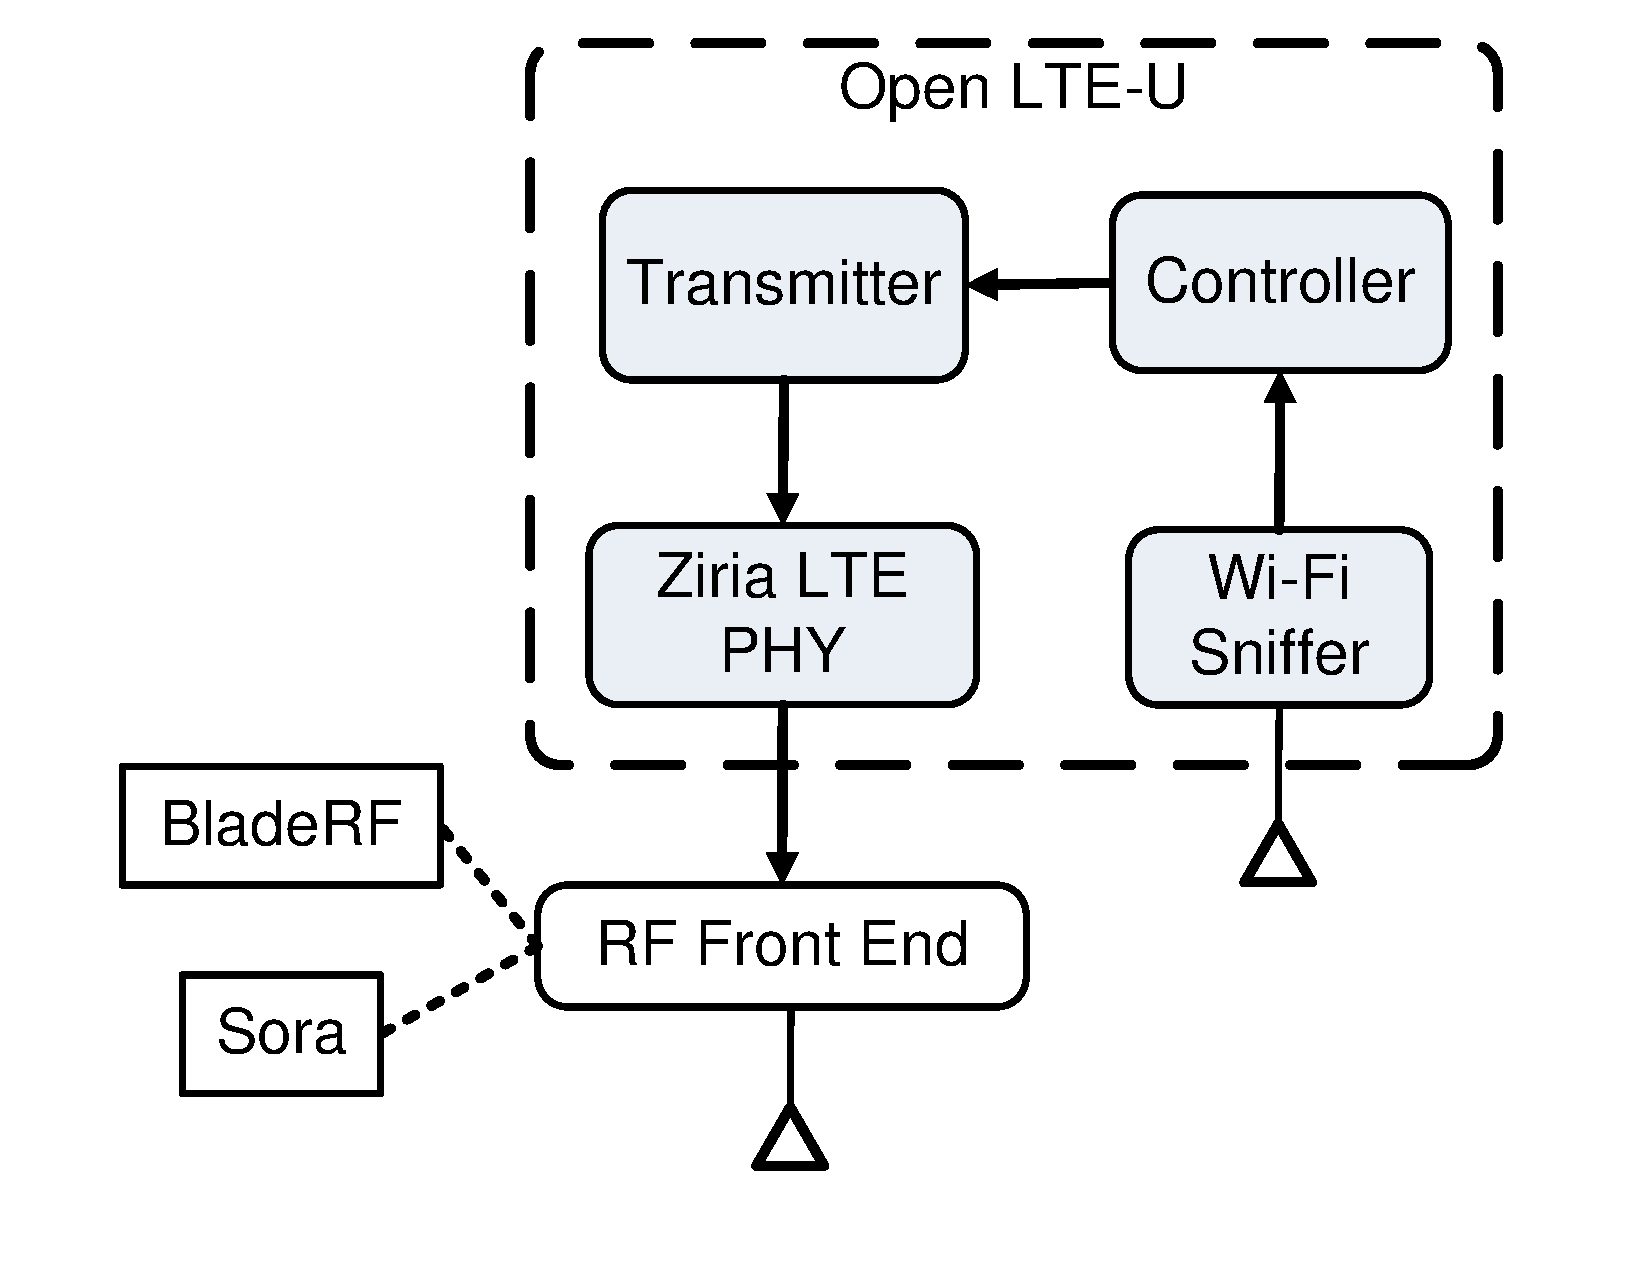
\includegraphics[width=2.4in]{./figures/architecture}
     \vspace{0.0cm}
     \caption{Architecture of Open LTE-U platform.}
   \label{fig:platform}
\end{figure}

\begin{figure}[!htb]
 \centering
     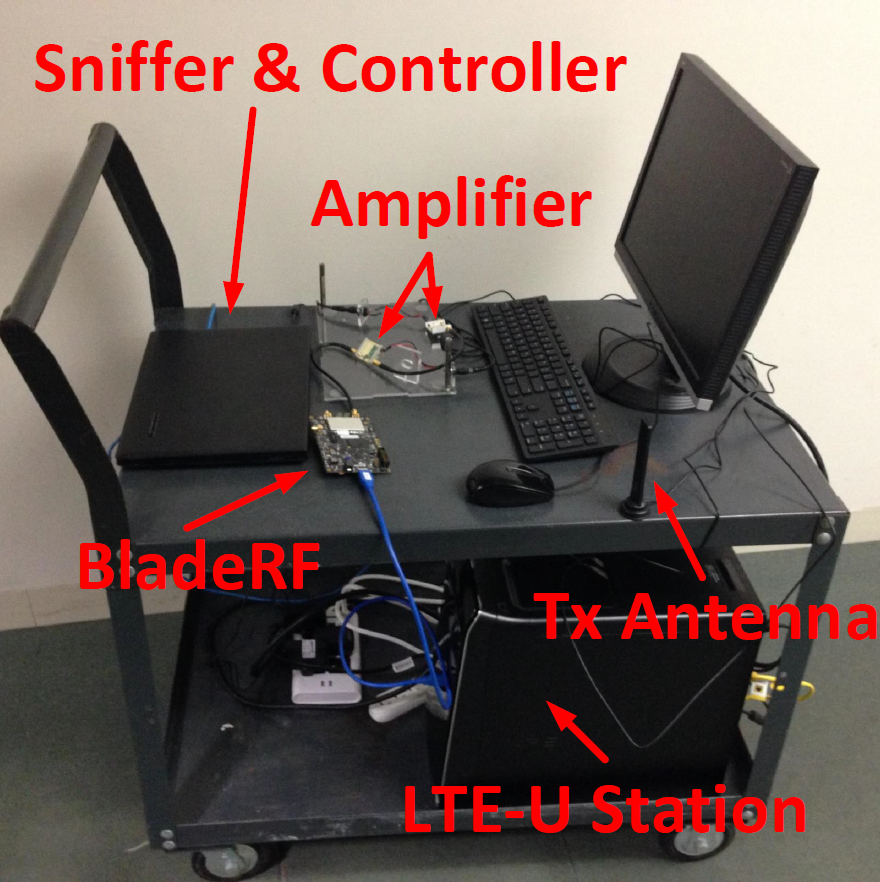
\includegraphics[width=1.6in]{./figures/testbed.png}
  \caption{The Open LTE-U testbed.}
   \label{fig:testbed}
\end{figure}


\subsection{LTE-U Base Station}


We have developed a fully functional LTE base-station (eNodeB) in-house, 
running on a programmable software-defined radio platform. 
To verify the correctness of our implementation, 
we tested it using commercial dongles in 700 MHz (commercial) bands, 
i.e., we create a synthetic downlink traffic load from the traffic observed in 700 MHz. 
Since Wi-Fi is running on unlicensed bands,  
we then adjusted the centre frequency and ran it in 2.4 GHz bands. 
Our radio platform currently doesn't support 5 GHz bands but since WiFi protocol is the same 
in 2.4 GHz and 5 GHz we don't expect different results. 
The output power of BladeRF device varies from frequency to frequency. 
We use two amplifier to increase the power to be around 15dBm,
which is the output power of most Wi-Fi access points we observed. 

The LTE-U base station can run in ``on'' and ``off'' mode. 
Ideally, there is LTE-U transmission when the base station
is running in ``on'' mode and no LTE-U trasmission when
it is running in ``off'' mode.
However, we observe strong DC offset on both Sora and BladeRF platforms. 
DC offset manifests itself as a large spike in the center of the spectrum. 
In the ``off'' period, the spike interferes with Wi-Fi 
transmissions. 
Due to hardware contraints, calibiration does not work well in this case. 
We use frequency hopping to emulate duty cycles. 
In ``off'' period, the LTE-U does not stop transmission, but
switch the centre frequency, so that the Wi-Fi 
links in current frequency bands are not affected. 
Switching to another band is not a perfect solution
and may lead other Wi-Fi links operating in that frequency
switch to another frequency, 
but we have not observed such scenarios in our measurement. 

\subsection{Wi-Fi Sniffer}


Sensing surrounding Wi-Fi transmissions is important for LTE-U to 
determine the duty cycles for fairness.
The Wi-Fi sniffer is a Wi-Fi traffic sensing mechanism for that. 
For example, if there is a single saturated Wi-Fi link, 
the duty cycle of LTE-U is supposed to be 50\%, 
i.e., either get half of the channel. 
Determining the duty cycle is a challenge problem. 
There are many saturated and unsaturated Wi-Fi links
in the air, and each Wi-Fi Access Point could
be connected by different number of Wi-Fi clients. 
It is challenging to define fairness in various conditions. 
The Wi-Fi sniffer is used to sensing the Wi-Fi links. 
It is able to capture the Wi-Fi packets in the air
and classify them into different links. 
By examining the medium utilization as well as
other parameters, the controller can determine 
the desired duty cycle. 
To this end, we bring up a monitor interface through
a Wi-Fi USB card. 
We use pcap library to decode the MAC and Physical
layer information. 
In each measurement interval (e.g., 10 duty cycles), 
the Wi-Fi sniffer push the sensed Wi-Fi 
packet (only the meta data) into a buffer. 
The buffer serves as the input for the controller. 
The buffer is cleared at each interval. 
The Wi-Fi sniffer is running on one software
thread on the Ubuntu machine. 

\subsection{Controller}

The controller is the policy that is used to adjust LTE-U duty cycles. 
It answers questions such as what is the desired duty cycles
given current medium utilization. 
One example policy is CSAT algorithm, 
which we will conduct analysis and illustrate measurement
results in later sections. 
The controller send control command through UDP socket
over Ethernet cable. 
The controller is one software thread that is running
on Ubuntu machine. 
The input of the controller is the Wi-Fi packet
buffer collected by the Wi-Fi sniffer.
By iterating over the Wi-Fi packets received during
last interval, we can calculate the Wi-Fi medium
utilization and number of Wi-Fi devices around. 
Based on these information, the controller
calculates the desired duty cycle for next interval
and send it to the LTE-U base station. 

